An elementary school teacher that lives in Sondrio has always loved mountain fauna. One day she decides to bring her students in a trip to show them the beauty of those creatures, so she connects to the website.\\
First she learns some basics about the association, then she proceeds to search for an interesting event during the current month that presents several services involving different animals. When she finds the best event for what she is looking for, she contacts the volunteer responsible for that event to reserve a place for her class.
	\begin{figure}[h!]
		\centering
		\begin{minipage}[b]{0.8\textwidth}
    			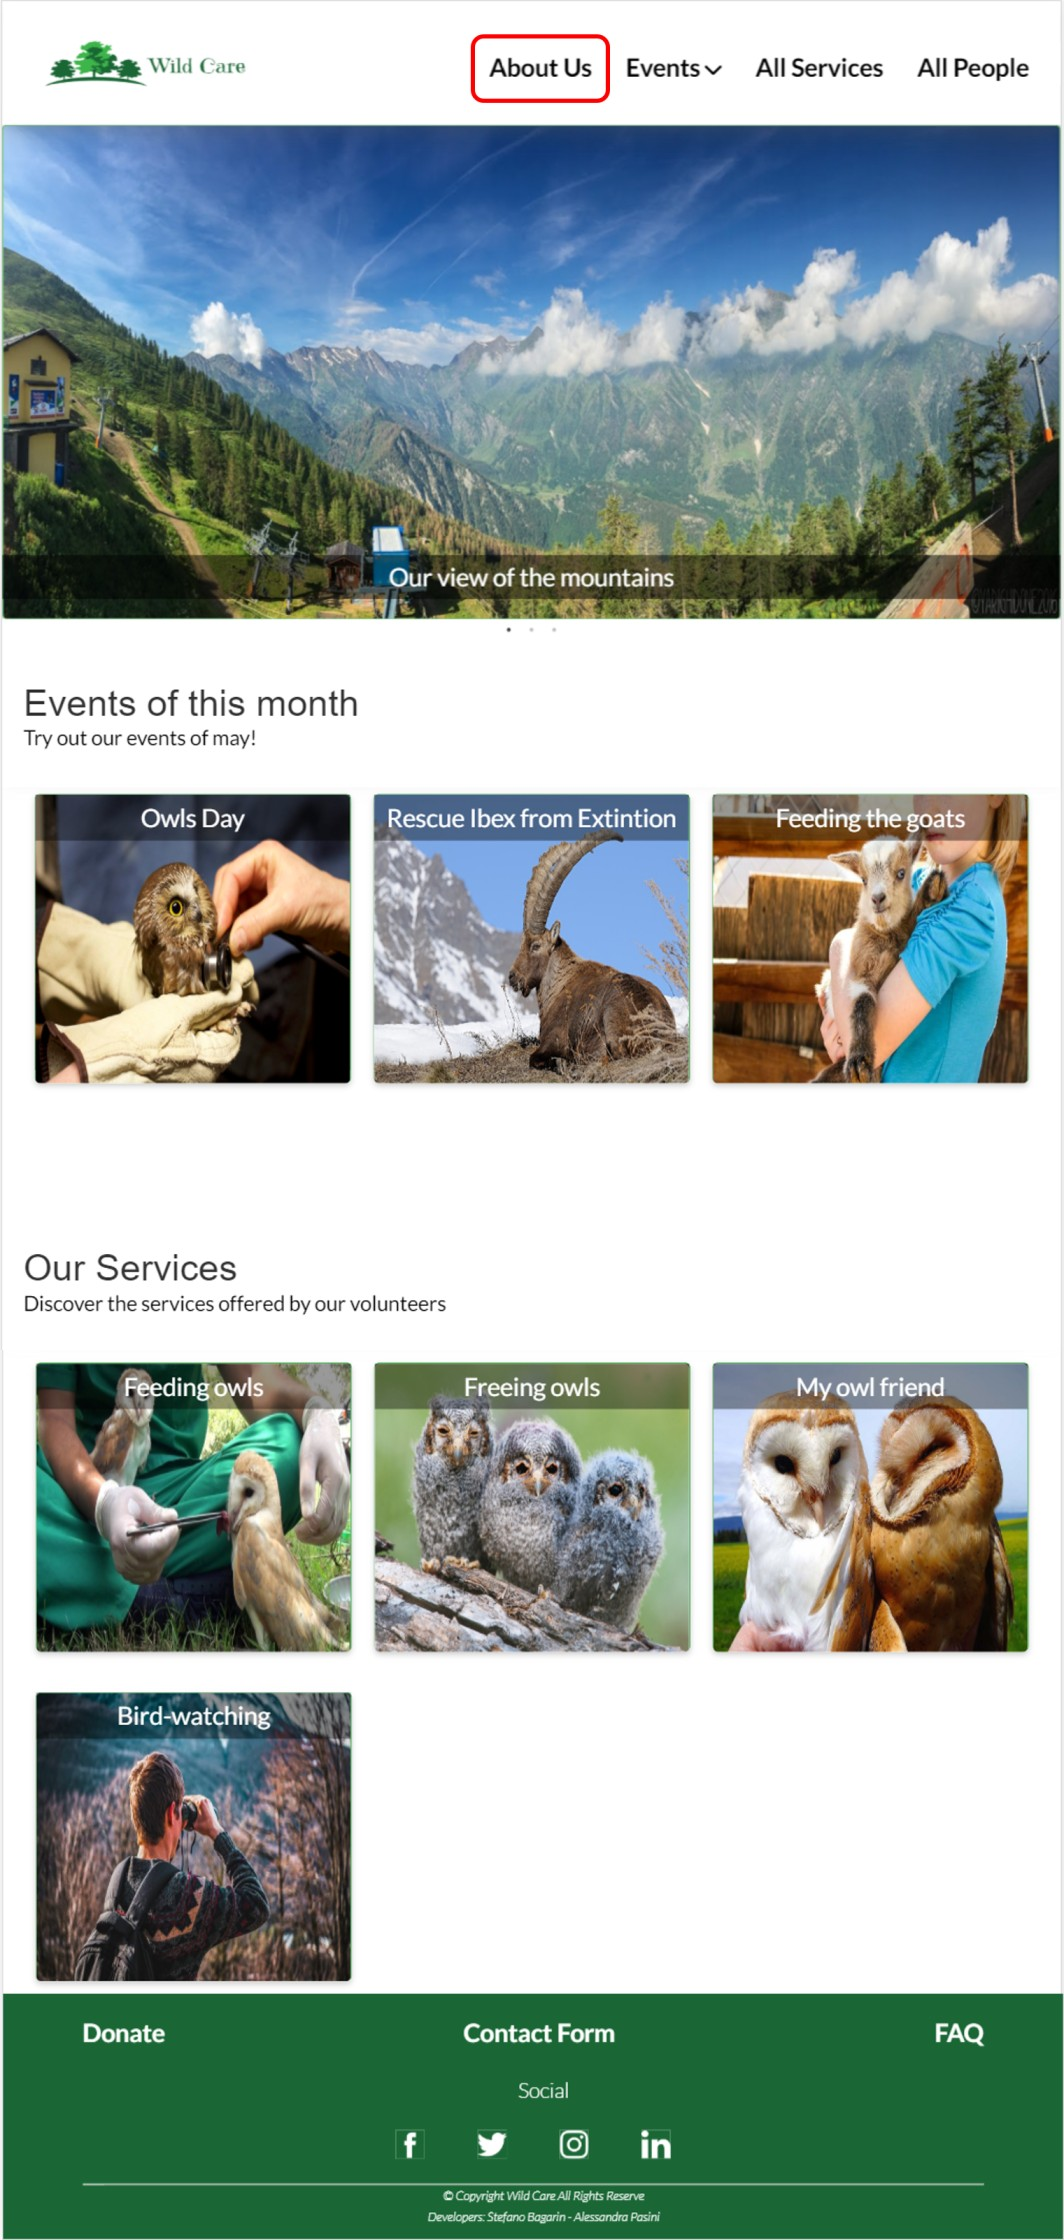
\includegraphics[width= \textwidth]{./assets/mockups/homepage_aboutus.jpg}
			\caption{Selects about us from the home page.}
		\end{minipage}
	\end{figure}

	\begin{figure}[h!]
		\centering
		\begin{minipage}[b]{1\textwidth}
    			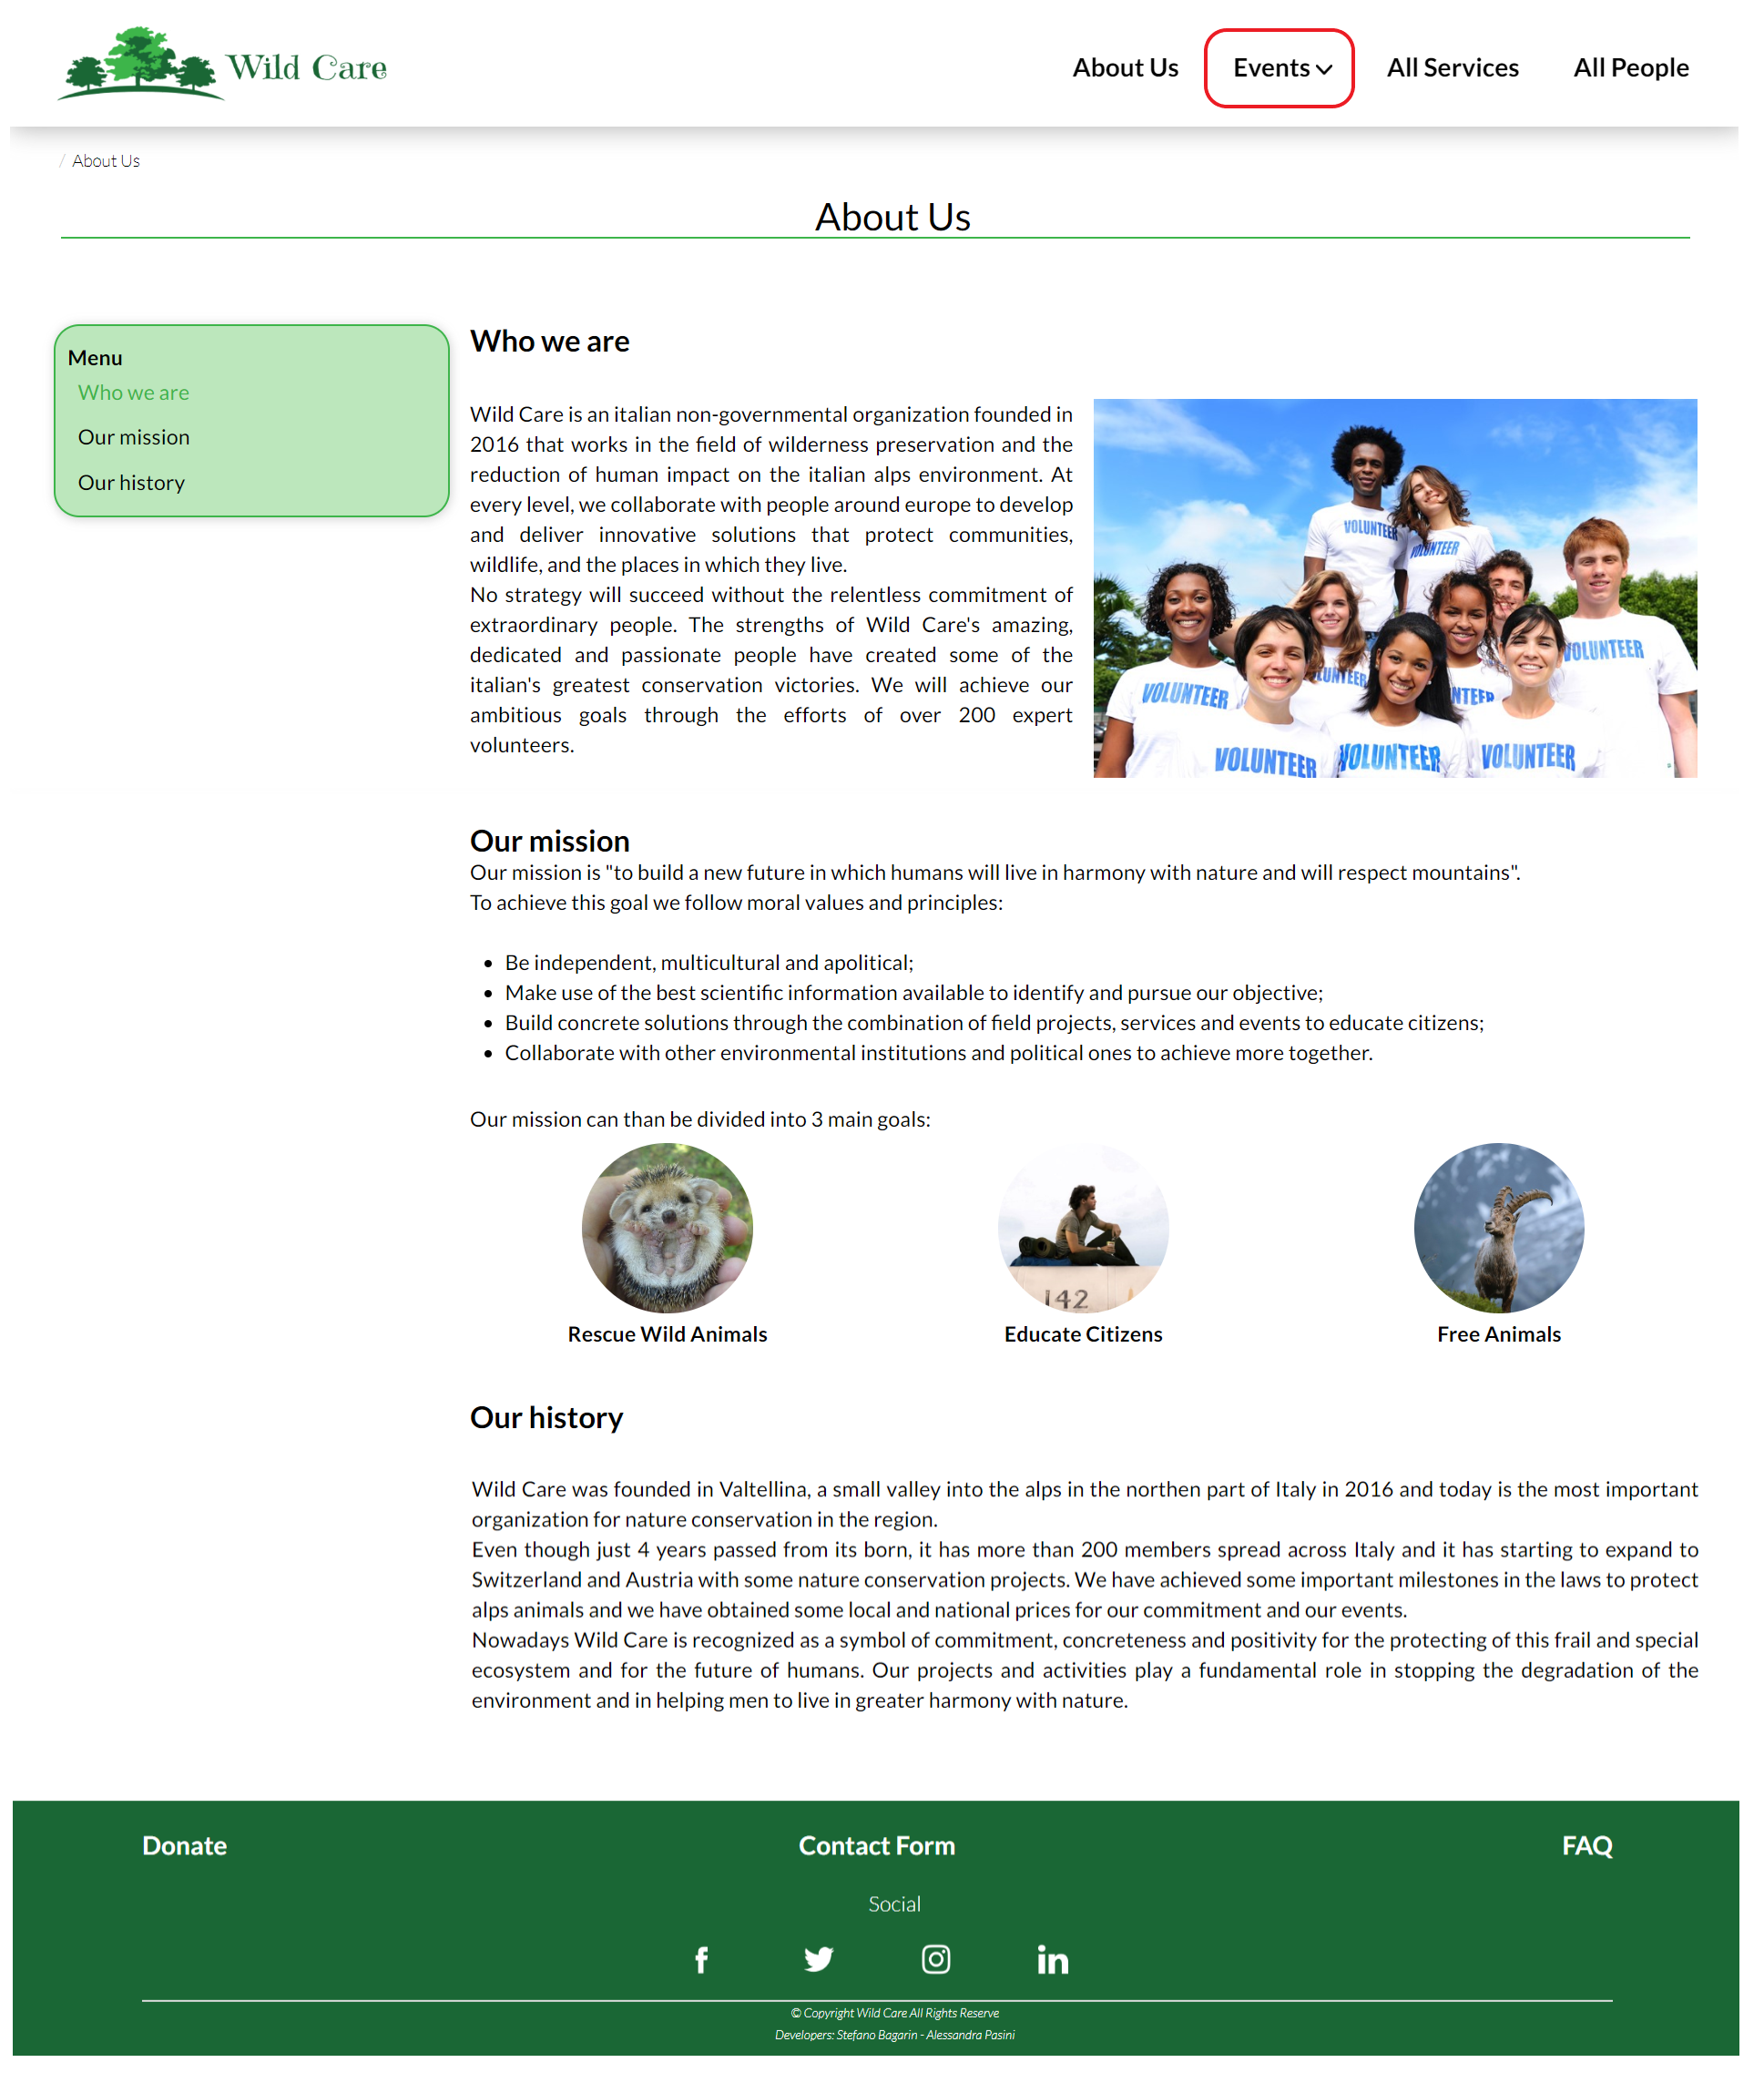
\includegraphics[width=\textwidth]{./assets/mockups/aboutus_eventsbymonth.png}
			\caption{Goes in the section events by month.}
		\end{minipage}
	\end{figure}

	\begin{figure}[h!]
		\centering
		\begin{minipage}[b]{1\textwidth}
    			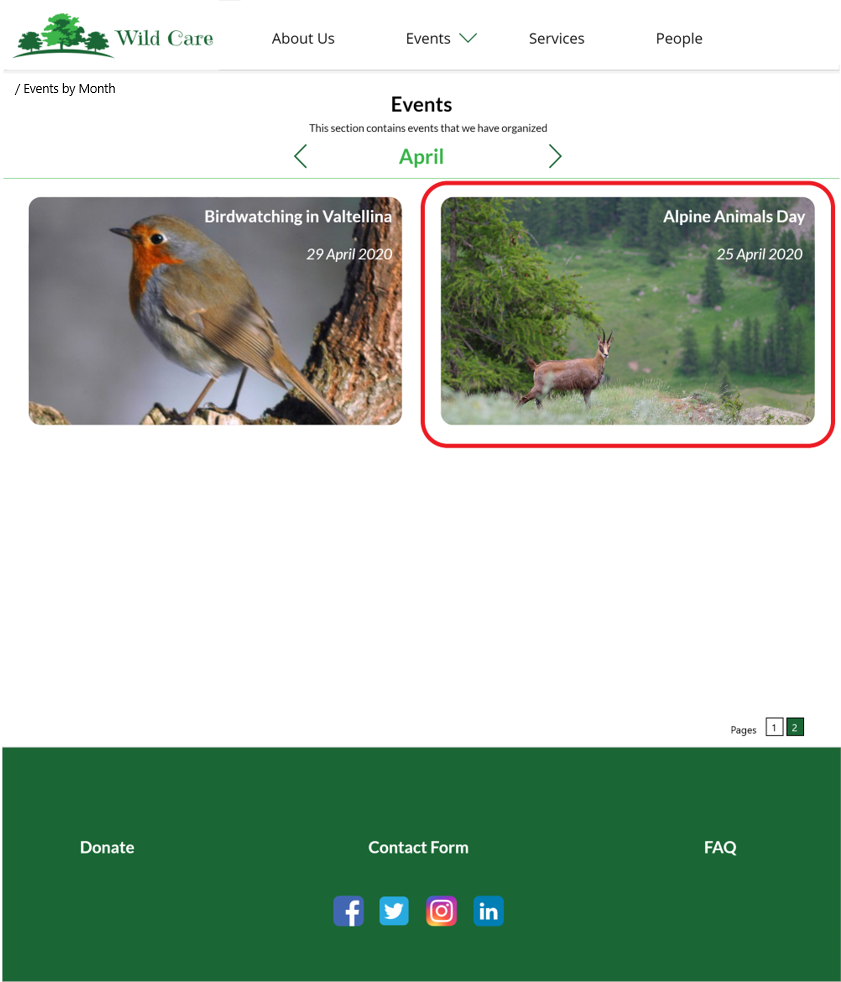
\includegraphics[width=\textwidth]{./assets/mockups/eventsbymonth_event.png}
			\caption{Selects an event.}
		\end{minipage}
	\end{figure}

	\begin{figure}[h!]
		\centering
		\begin{minipage}[b]{1\textwidth}
    			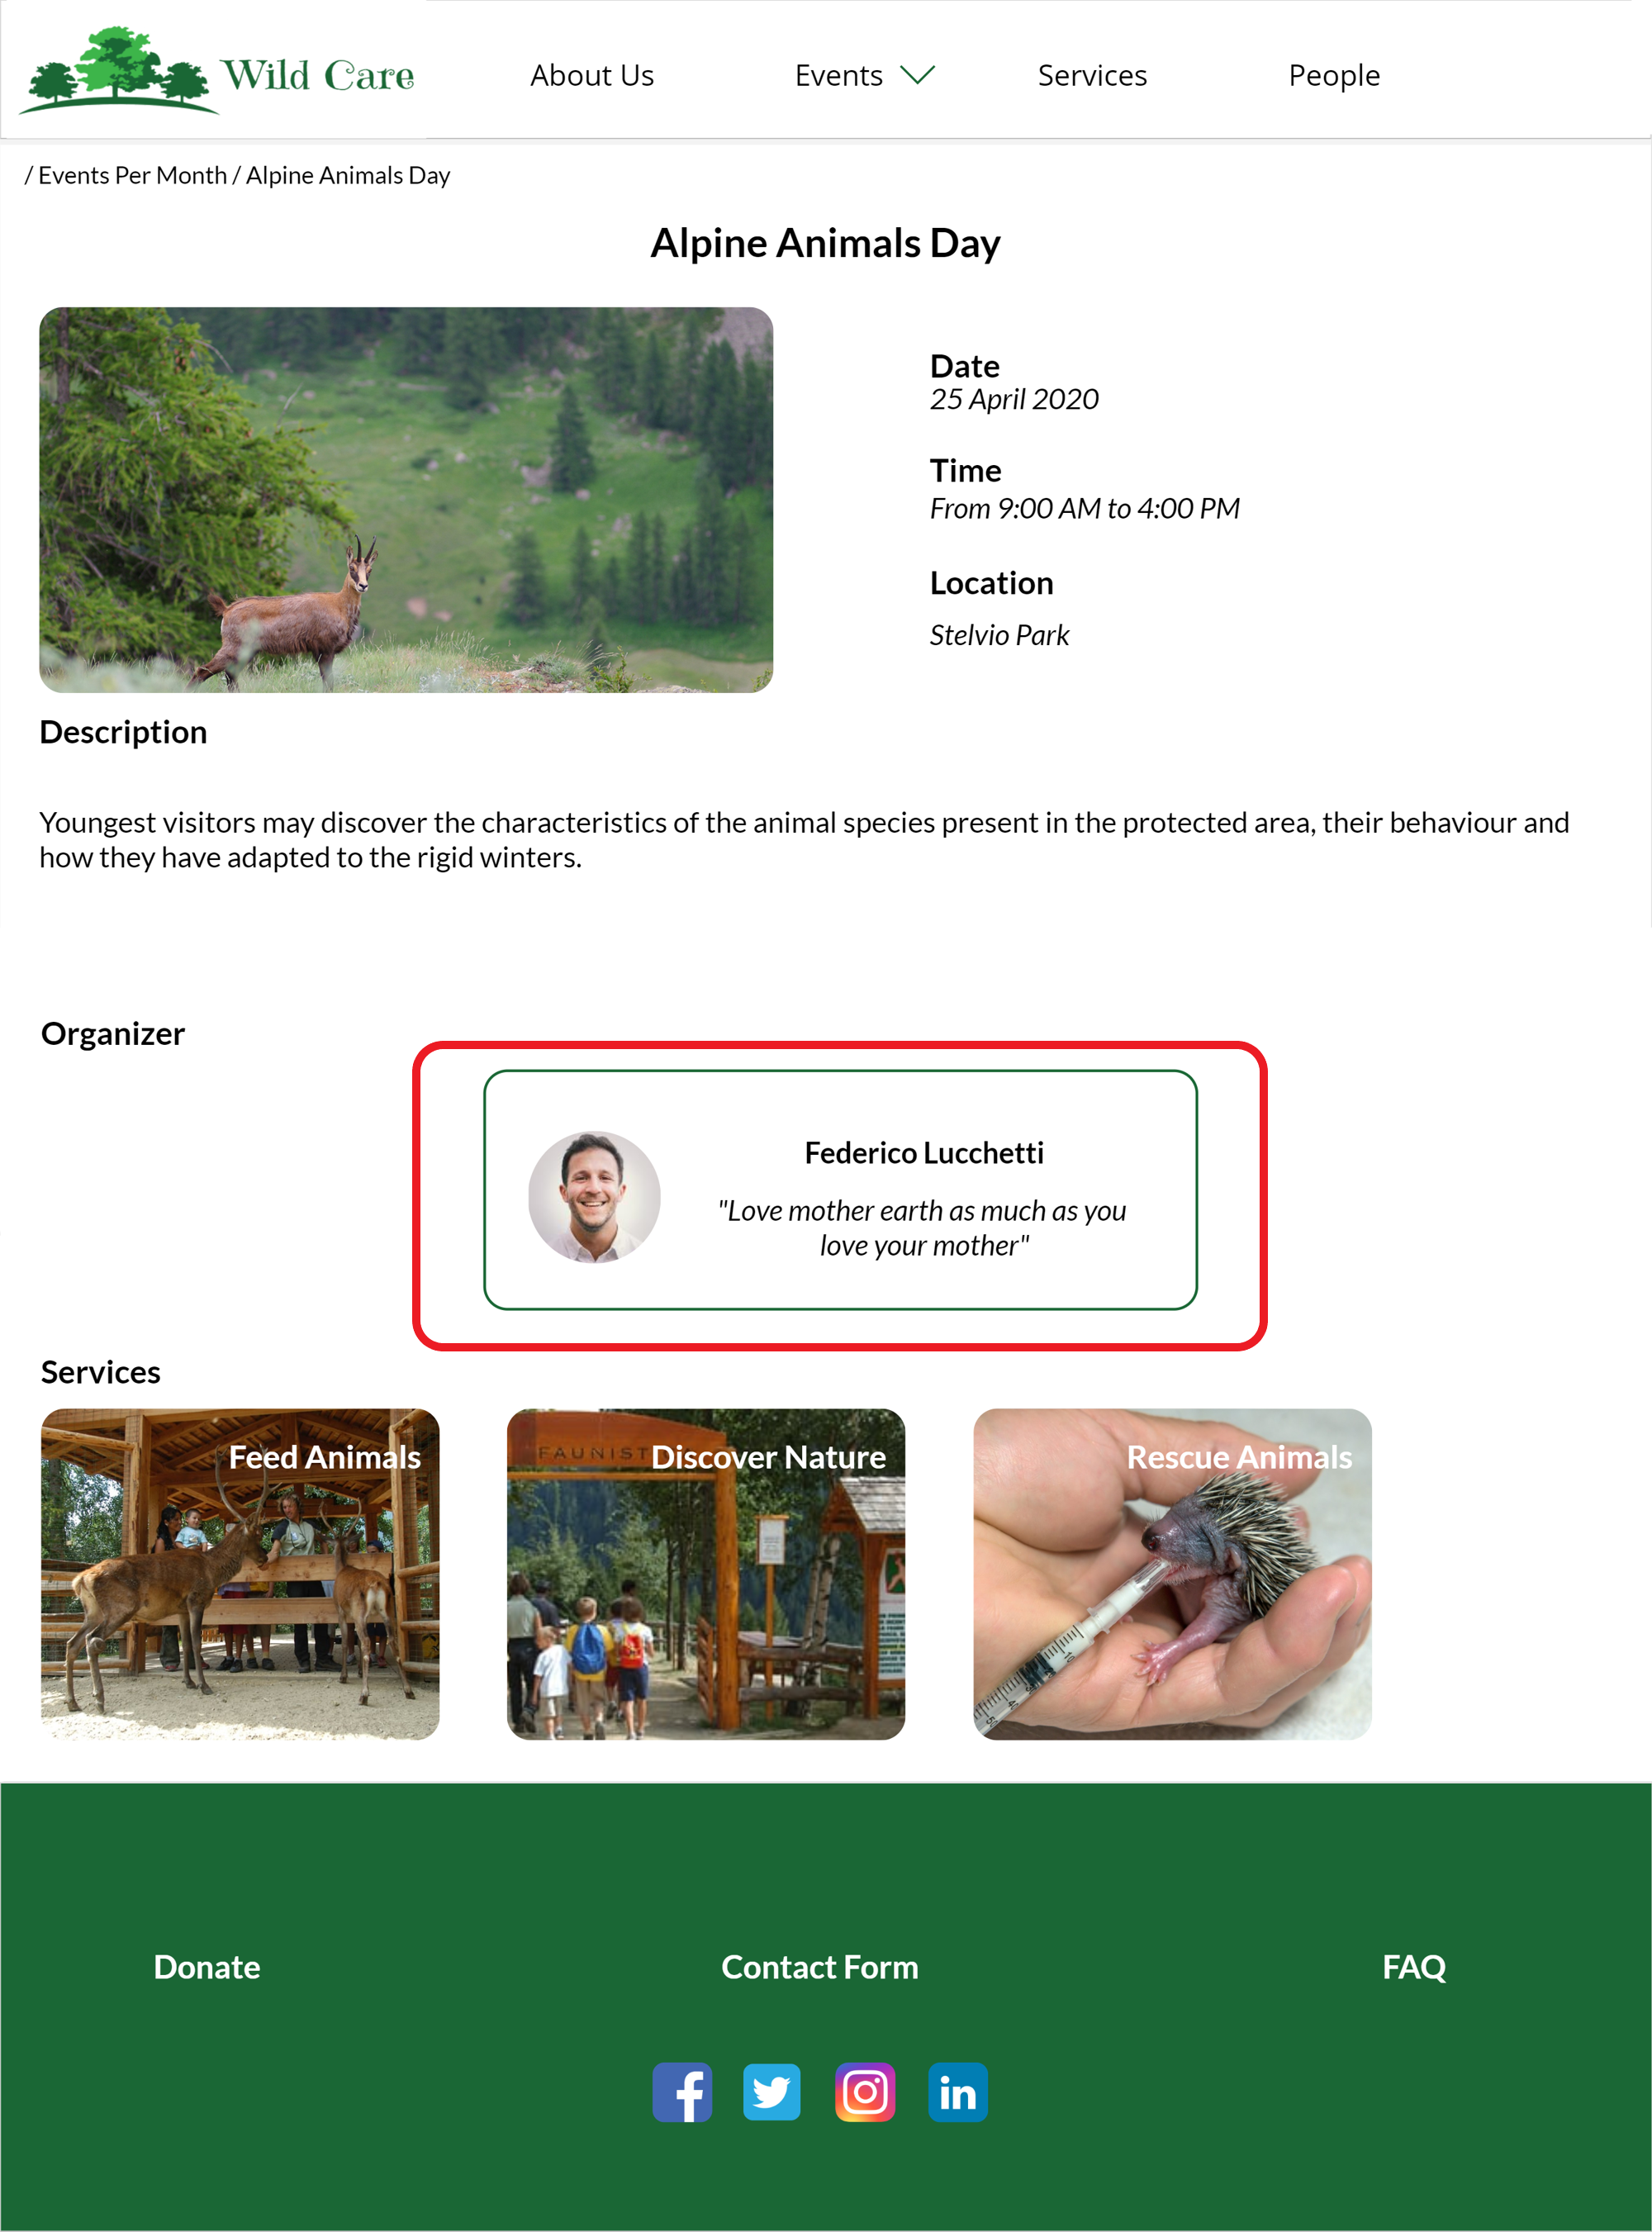
\includegraphics[width=\textwidth]{./assets/mockups/eventdetails_persondetails.png}
			\caption{Goes to the page of the responsible of the event.}
		\end{minipage}
	\end{figure}

	\begin{figure}[h!]
		\centering
		\begin{minipage}[b]{1\textwidth}
    			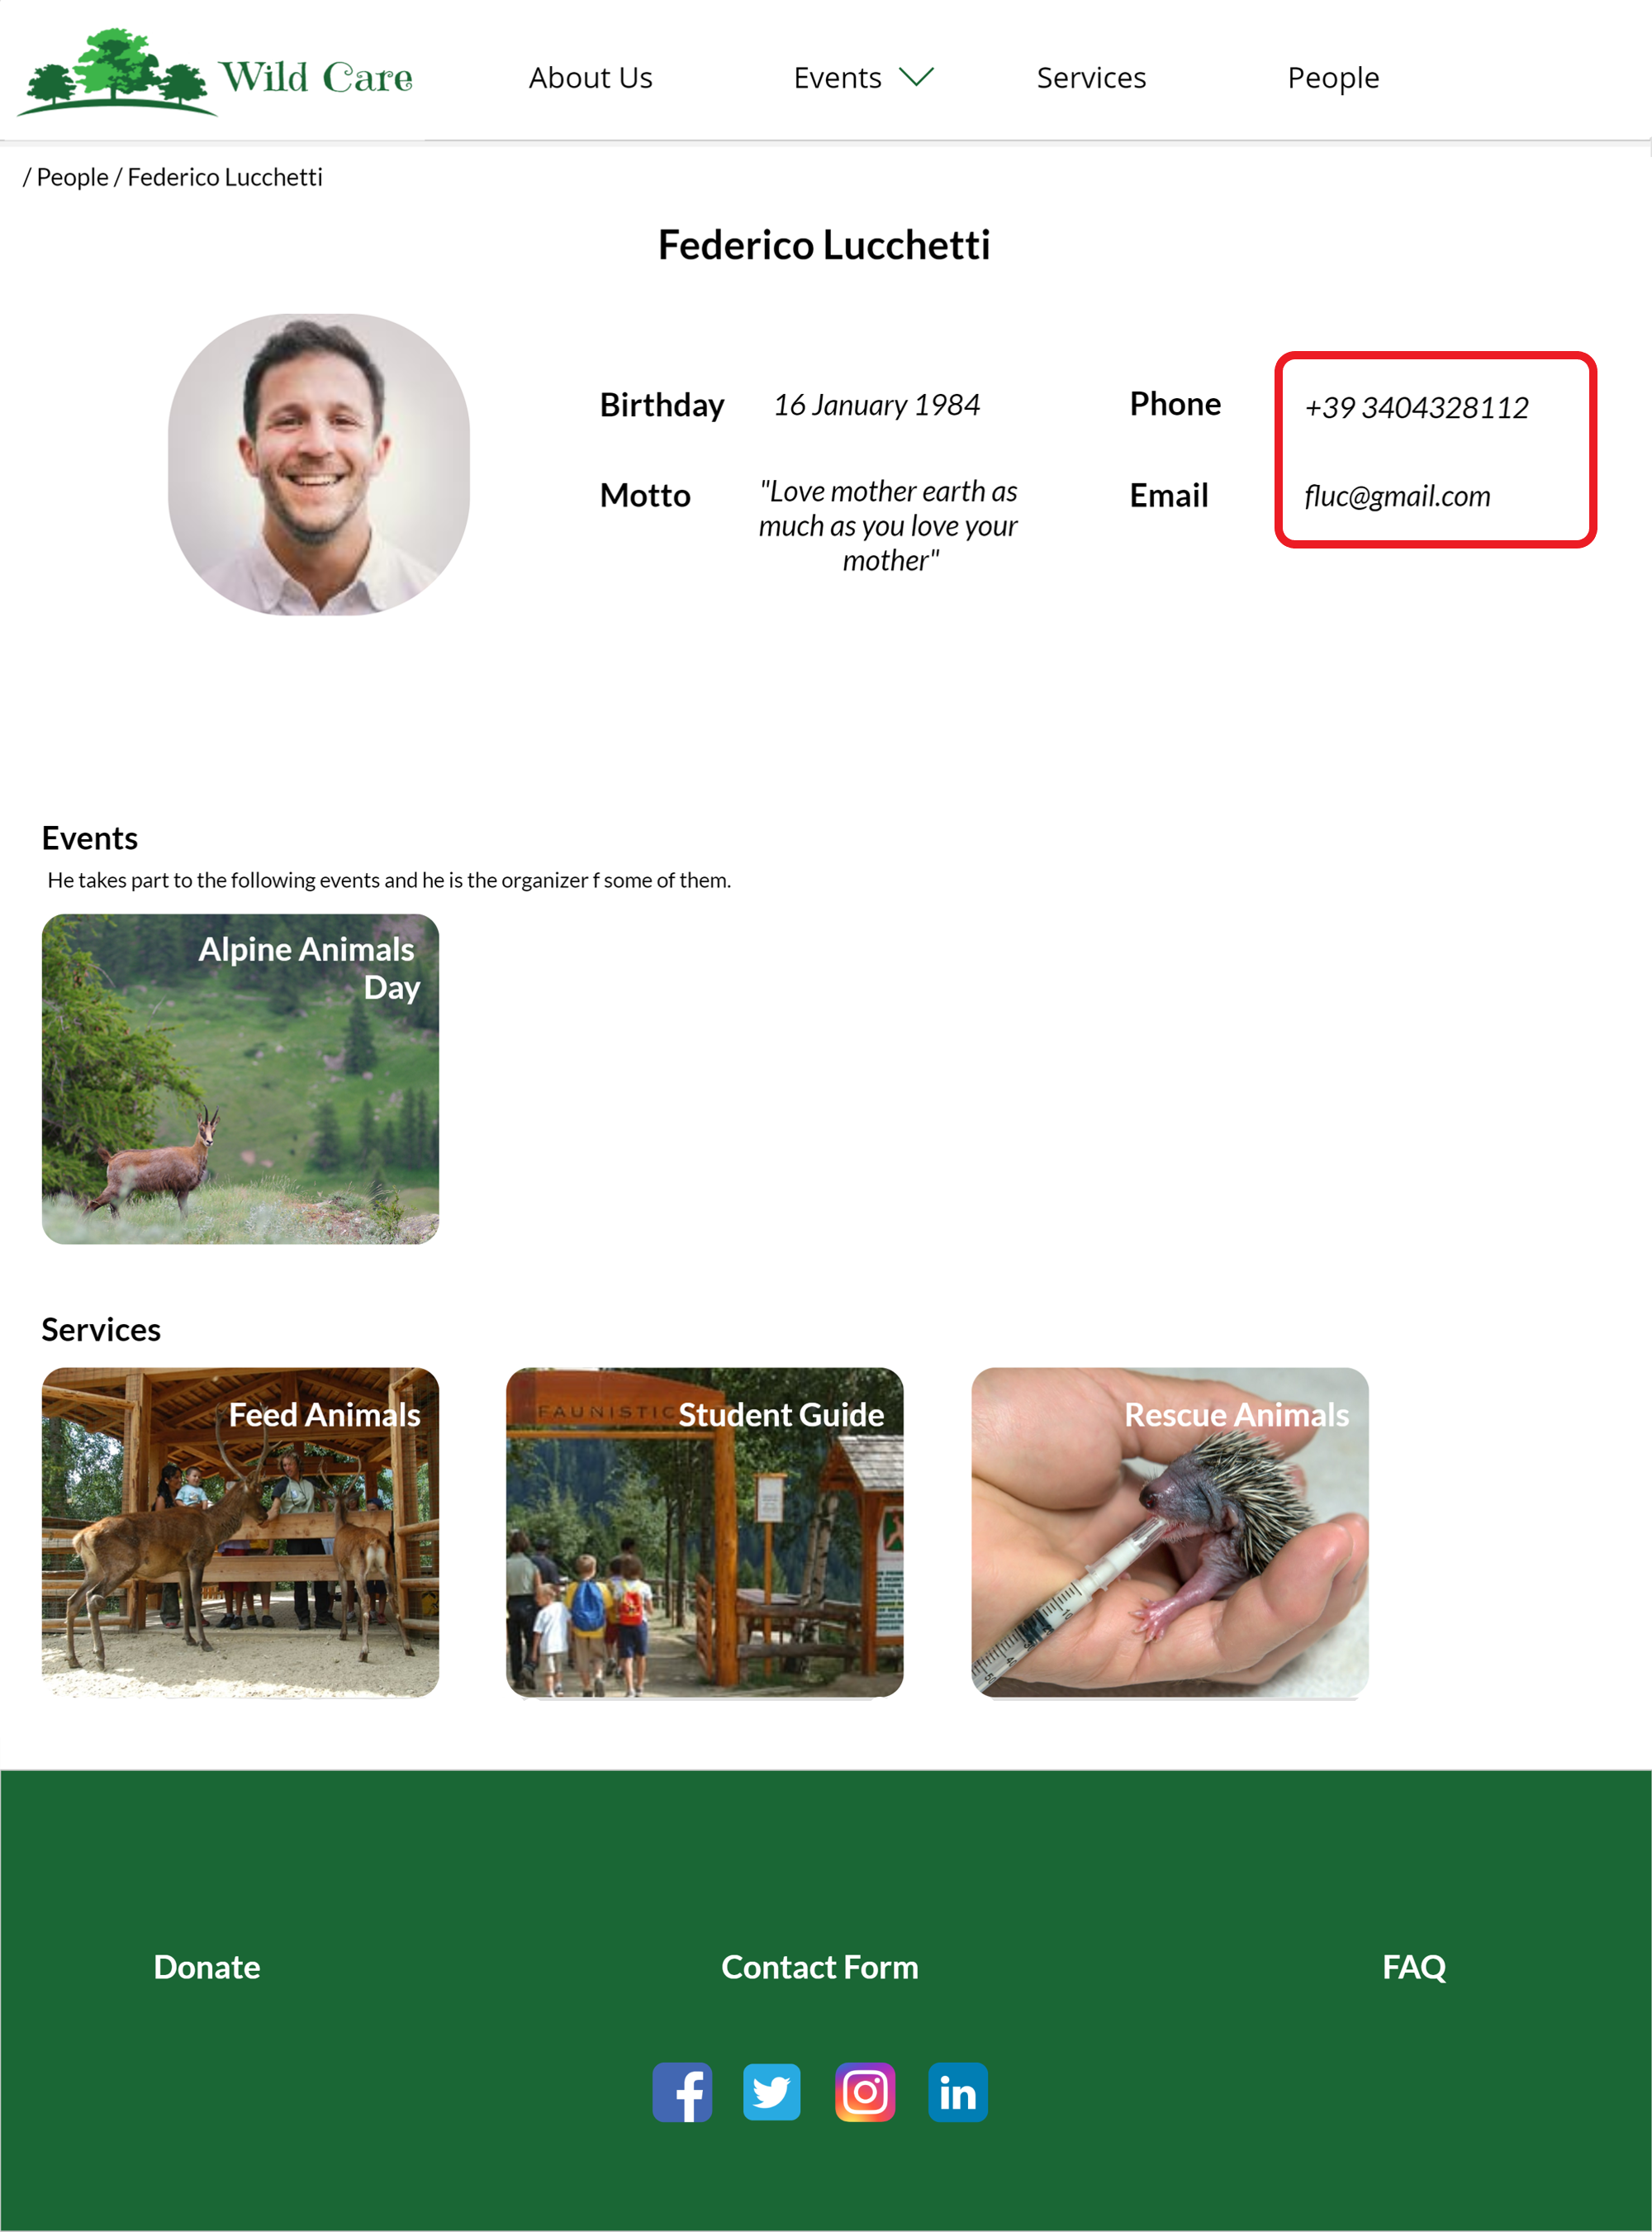
\includegraphics[width=\textwidth]{./assets/mockups/persondetails_contacts.png}
			\caption{Takes the email or the phone number of the responsible to contact it.}
		\end{minipage}
	\end{figure}